\documentclass{article}
\usepackage{amsmath}
\usepackage{amssymb}
\usepackage{algpseudocode}
\usepackage{algorithm}
\usepackage{listings, listings-rust}
\usepackage{biblatex}
\addbibresource{refs.bib}

%Hi Caio, very nice! But, now, as I understand it, there is a runtime
%check whenever you create an object. What's the cost of this runtime
%check? Could you create a large number of objects (never modifying
%them), to see the cost? Try two setups:
%
%C. Lots of collisions in the table.
%N. No collision.
%
%Then you can do {with check | without check} * {C | N}. This setup
%will give you four lines. Each line can be formed by varying the
%number of objects created. What do you think?

\usepackage{xfrac,unicode-math}
\defaultfontfeatures{Scale=MatchLowercase}

\setmainfont{Libertinus Serif}
\setmathfont{Libertinus Math}
\setmonofont{Go Mono}


\setlength{\parindent}{0pt}
\newcommand*\compl[1]{\overline{#1}}
\makeatletter
\newcommand{\fixed@sra}{$\vrule height 2\fontdimen22\textfont2 width 0pt\shortrightarrow$}
\newcommand{\shortarrow}[1]{%
  \mathrel{\text{\rotatebox[origin=c]{\numexpr#1*45}{\fixed@sra}}}
}
\makeatother

\begin{document}

\section{Motivation}

Memoizing objects in Python is quite easy. However, the following program has a semantic error.

\begin{lstlisting}[language=Python, style=boxed, tabsize=2]
from functools import cache

@cache
class Person:
    def __init__(self, name, age):
        self.name = name
        self.age = age

p0 = Person("Michael", 31)
p1 = Person("Michael", 31) # p1 == p0 due to memoization
p1.name = "Caio"
p1.age = 22

print(p0.name, p0.age)
print(p1.name, p1.age)
\end{lstlisting}

As \textit{p0} and \textit{p1} point to the same object in memory, the program produces the unsatisfactory output:

\begin{lstlisting}[style=boxed]
Caio 22
Caio 22
\end{lstlisting}

\section{Description of the Alias Set Algorithm}

Consider the following Hush program, where \texttt{Point} and \texttt{Triangle} are memoized.

\begin{lstlisting}[language=Rust, style=boxed, tabsize=2]
let p0 = Point(1, 1)
let p1 = Point(1, 1) // p1 -> p0 due to memoization
let p2 = p1

let t0 = Triangle(p0, p1, p2)
\end{lstlisting}

Analogous to the Python example, this program can be invalidaded if we change \textit{p0}, \textit{p1} or \textit{p2}, as they all point to the same object in memory. However, by using an \textit{alias set} we can keep track of references and instatiate new objects when we see fit.

\begin{figure}[h]
\centering
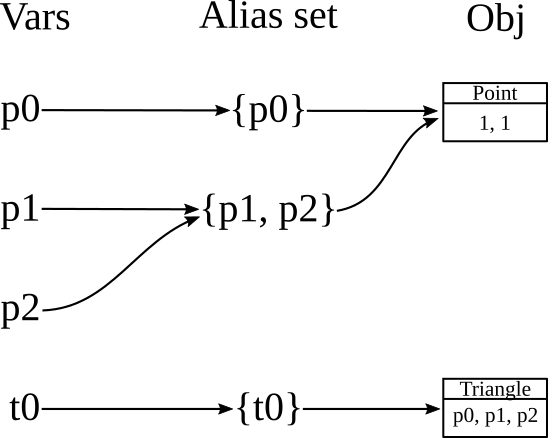
\includegraphics[width=6cm]{alias-set-diagram.png}
\caption{Memory layout of Program 2}
\end{figure}

\section{Current State of Memoization in Hush}
\begin{itemize}
	\item We have memoization and objects as closures $\to$ We can memoize immutable objects.
	\item Raise exception when mutating memo objects. [DONE]
	\item Memoization of arbitrary objects. [WIP]
\end{itemize}

\printbibliography

\end{document}
